% !TEX root = webmatematik.tex

\section{Multipel regression}

\subsection{Introduktion}
Fra simpel \href{http://www.webmatematik.dk/lektioner/matematik-b/regression}{lineær regressions} analyse ved vi, hvordan man med \href{http://www.webmatematik.dk/lektioner/matematik-b/regression}{mindste kvadraters metoden} bestemmer den lineære funktion, som bedst passer til en række observationer i 2D planen.

Vi har altså her observationer \((y_i, x_i)\) for \(i=1,\ldots,n\) og ønsker at bestemme konstanterne \(a\) og \(b\) på en sådan måde, at den lineære funktion
\begin{displaymath}
  y = a + b x
\end{displaymath}
ligger så tæt på alle observationer \((y_i, x_i)\) som muligt.

Verden er dog sjældent så simpelt indrettet, at man kan beskrive en \textit{afhængig} variabel \(y\) med kun en enkelt \textit{forklarende} variabel \(x\).

Multipel regression er en udvidelse af simpel regression, hvor vi i stedet for en enkelt for\-kla\-ren\-de variabel har to eller flere forklarende variable. For\-kla\-ren\-de variable kaldes til tider også for \textit{kovarianter} mens afhængige variable somme tider omtales som \textit{respons} variable.

\subsection{Model}
Vi har \(n\) observationer \(y_i,x_{i1},x_{i2},\ldots,x_{ip}\) hvor \(i=1,\ldots,n\) og ønsker at bestemme konstanter \(b_0,b_1,b_2,\ldots,b_p\), så funktionen
\begin{displaymath}
  y = b_0 + b_1 x_1 + b_2 x_2 + \cdots b_p x_p
\end{displaymath}
ligger så tæt på alle punkterne \(y_i,x_{i1},x_{i2},\ldots,x_{ip}\) som muligt. Konstanterne kaldes for regressionskoefficienterne.

Bemærk, at der nu er et dobbelt indeks på \(x\)'erne. Det er nødvendigt, da vi nu har \(p\) forklarende variable istedet for blot en enkelt forklarende variabel. Så når vi skriver
\begin{displaymath}
  x_{ij}, \quad i=1,\ldots,n \quad \textrm{ og } \quad j=1,\ldots,p
\end{displaymath}
er der tale om den \(j\)'te forklarende variable for den \(i\)'te observation.
Vi kan stille observationerne op i en tabel
\begin{table}[h]
\centering
\caption{Oversigt over observationer}
\label{my-label}
\begin{tabular}{cccccc}
\hline
\multicolumn{1}{l}{Observation} & \multicolumn{1}{l}{\begin{tabular}[c]{@{}l@{}}Afhængig\\ variabel\end{tabular}} & \multicolumn{4}{c}{Forklarende variable}          \\ \hline
                                & \(Y\)                                                                           & \(X_1\)    & \(X_2\)    & \(\cdots\) & \(X_p\)    \\ \hline
1                               & \(y_1\)                                                                         & \(x_{11}\) & \(x_{12}\) & \(\cdots\) & \(x_{1p}\) \\ \hline
2                               & \(y_2\)                                                                         & \(x_{21}\) & \(x_{22}\) & \(\cdots\) & \(x_{2p}\) \\ \hline
3                               & \(y_3\)                                                                         & \(x_{31}\) & \(x_{32}\) & \(\cdots\) & \(x_{3p}\) \\ \hline
\(\vdots\)                      & \(\vdots\)                                                                      & \(\vdots\) & \(\vdots\) & \(\vdots\) & \(\vdots\) \\ \hline
n                               & \(y_n\)                                                                         & \(x_{n1}\) & \(x_{n2}\) & \(\cdots\) & \(x_{np}\) \\ \hline
\end{tabular}
\end{table}
for på den måde at vise, at vi har \(p\) forklarende variable og \(n\) observationer.
Regressionskoefficienter bliver normal fundet (estimeret) ved brug af mindste kvadrater metoden, dvs man vælger \(b_0, b_1, \ldots , b_p\)  således at udtrykket
\begin{equation}\label{eq:sse}
  SSE =\sum^n_{i=1} {\big(y_i - b_0 - b_1 x_{i1} - b_2 x_{i2} - \cdots - b_p x_{ip} \big)}^2
\end{equation}
minimeres. SSE er engelsk for Sum of Squares Errors. Dette er samme fremgangsmetode som kendes fra simpel lineær regression. \(b_0\) kaldes for skæringen og de øvrige \(b\)'er kaldes hældninger.

Formlen for koefficienterne \(b_0,b_1,b_2,\ldots,b_p\) er noget mere kompliceret i det generelle tilfælde, så den springer vi over her. Men nedenfor gennengår vi et eksempel på, hvordan man kan bestemme koefficienter ved brug af Microsoft Excel.

\subsection{Residualer}
Når vi har bestemt regressionskoefficienterne \(b_0,b_1,b_2,\ldots,b_p\) så kan vi udregnede de \textit{fittede} værdier for observationerne \(x_{i1},x_{i2},\ldots,x_{ip}\) hvor \(i=1,\ldots,n\). For den \(i\)'te observation er den fittede værdi
\begin{displaymath}
  \widehat{y_i} = b_0 + b_1 x_{i1} + b_2 x_{i2} + \cdots b_p x_{ip}
\end{displaymath}
og vi definerer residualer som værende forskellen \(e_i\) mellem observationen \(y_i\) og den fittede værdi \(\widehat{y_i}\)
\begin{displaymath}
  e_i = y_i - \widehat{y_i}
\end{displaymath}
Bemærk at ligning \ref{eq:sse} også kan skrives
\begin{displaymath}
  SSE =\sum^n_{i=1} {\big(y_i - b_0 - b_1 x_{i1} - b_2 x_{i2} - \cdots - b_p x_{ip} \big)}^2 = \sum^n_{i=1} {\big(y_i - \widehat{y_i} \big)}^2 =  \sum^n_{i=1} {e_i}^2
\end{displaymath}
så når vi finder minimum for \(SSE\), så minimerer vi residualerne eller med andre ord - forskellen mellem de observerede og fittede værdier.

\subsection{Visualisering af løsningen}
I tilfældet med simpel regression bestemmer vi en ret linie som passer bedst til observationerne. Det er umuligt at visualisere multipel regression i det generelle tilfælde. For det særlige tilfælde, hvor vi har to forklarende variable \(x_1\) og \(x_2\) og dermed modellen
\begin{displaymath}
  y = b_0 + b_1 x_1 + b_2 x_2
\end{displaymath}
så kan vi stadig visualisere løsningen. Vi kan tænke på observationerne \((x_{i1}, x_{i2}, y_i), i=1,\ldots,n\) som punkter i rummet, dvs i 3D koordinatsystemet med akser \(X_1, X_2\) og \(Y\).
\begin{center}
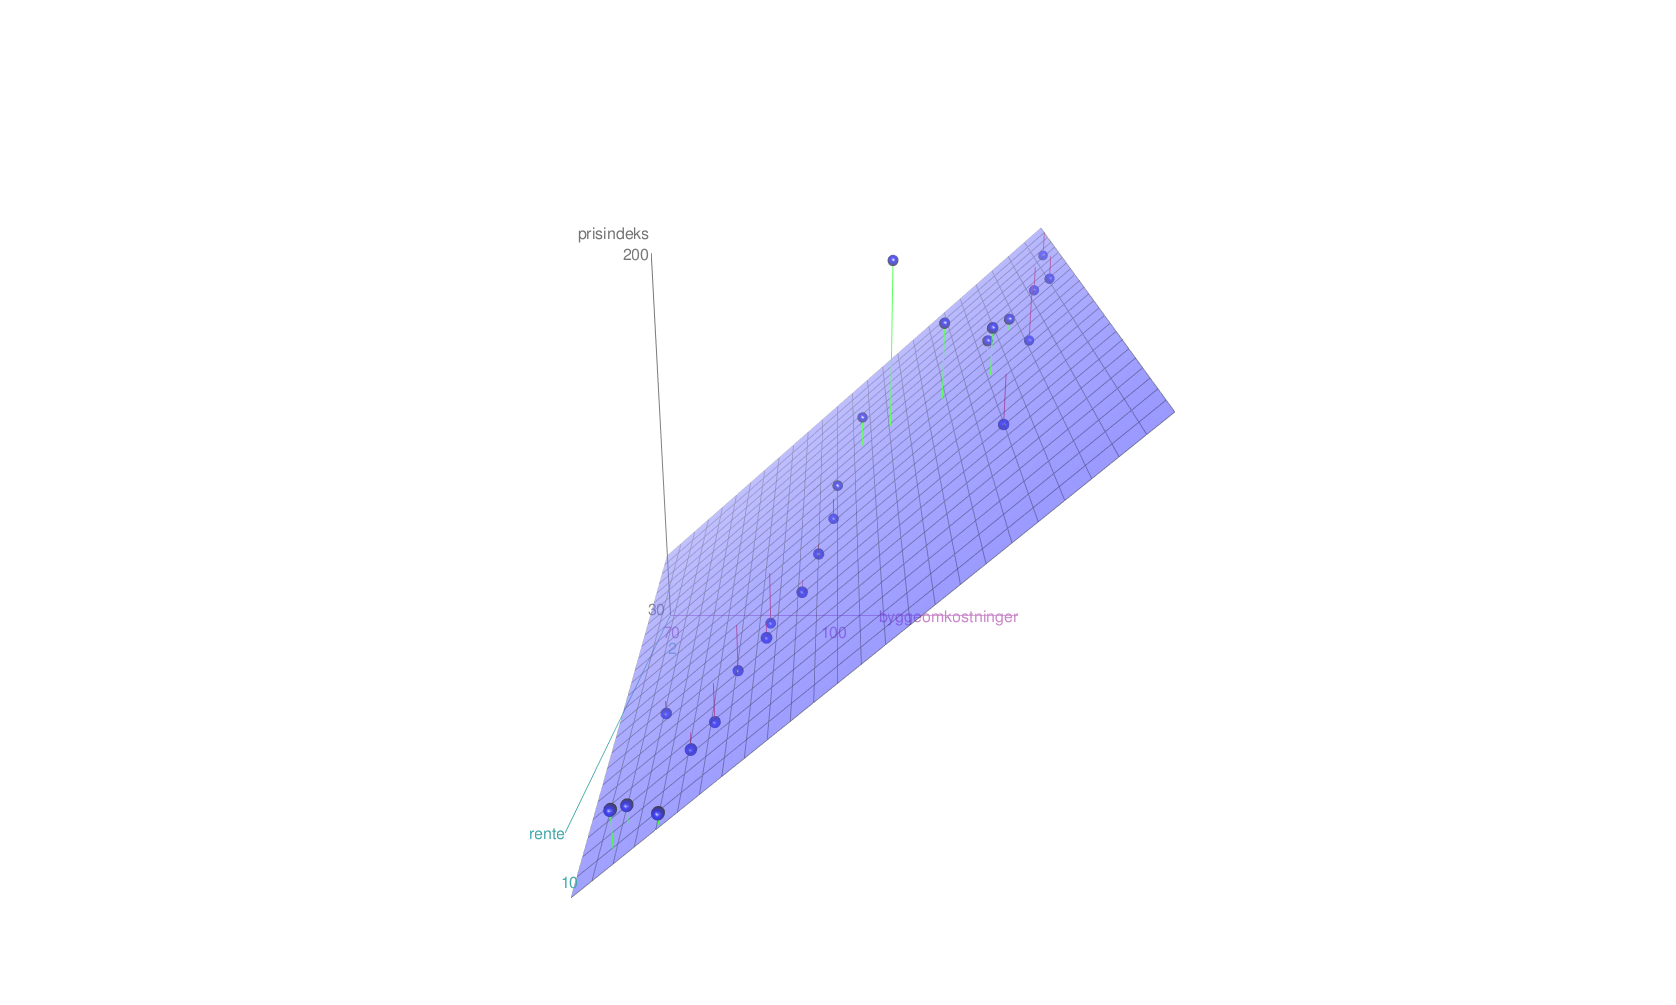
\includegraphics[height=12cm]{regression/images/visualisering.JPG}
\end{center}
Løsningen er nu ikke længere en ret linie, men derimod den plan som ligger tættest på alle punkterne. På figuren kan vi også se residualerne - de er plottet som linier mellem observationerne og planen. Nogle observationer ligger over planen og er markeret med en grøn linie, mens andre observartioner ligger under planen og er markeret med en rød linie.

\subsection{Prognoser - TODO}
Hvis koefficienterne \(b_0,b_1,b_2,\ldots,b_p\) er kendt, kan vi bruge formlen
\begin{displaymath}
\hat{y} = b_0 + b_1 x_1 + b_2 x_2 + \cdots + b_p x_p
\end{displaymath}
til at forudsige
hvad bruger vi regression til - forudsige

\subsection{Eksempel}
Lad os se på et (simplificeret) eksempel på multipel regressionsanalyse. Eksemplet er hentet fra opgaven \href{http://studenttheses.cbs.dk/xmlui/handle/10417/6138}{``Prisdannelse på ejerlejligheder i København''}  af Vibeke Stål og Anne Melvej Stennevad. Forfatterne undersøger, om der er en lineær sammenhæng mellem prisen på ejerlejligheder i København og en række faktorer såsom fx rente og byggeomkostninger.
\begin{displaymath}\label{eq:model}
  \textrm{prisindeks} = b_0 + b_1 * \textrm{byggeomkostninger} + b_2 * \textrm{rente}
\end{displaymath}
Hvordan bestemmer man regressionskoefficienterne \(b_0, b_1\) og \(b_2\), hvis vi har observationer som vist her i Excel
\begin{center}
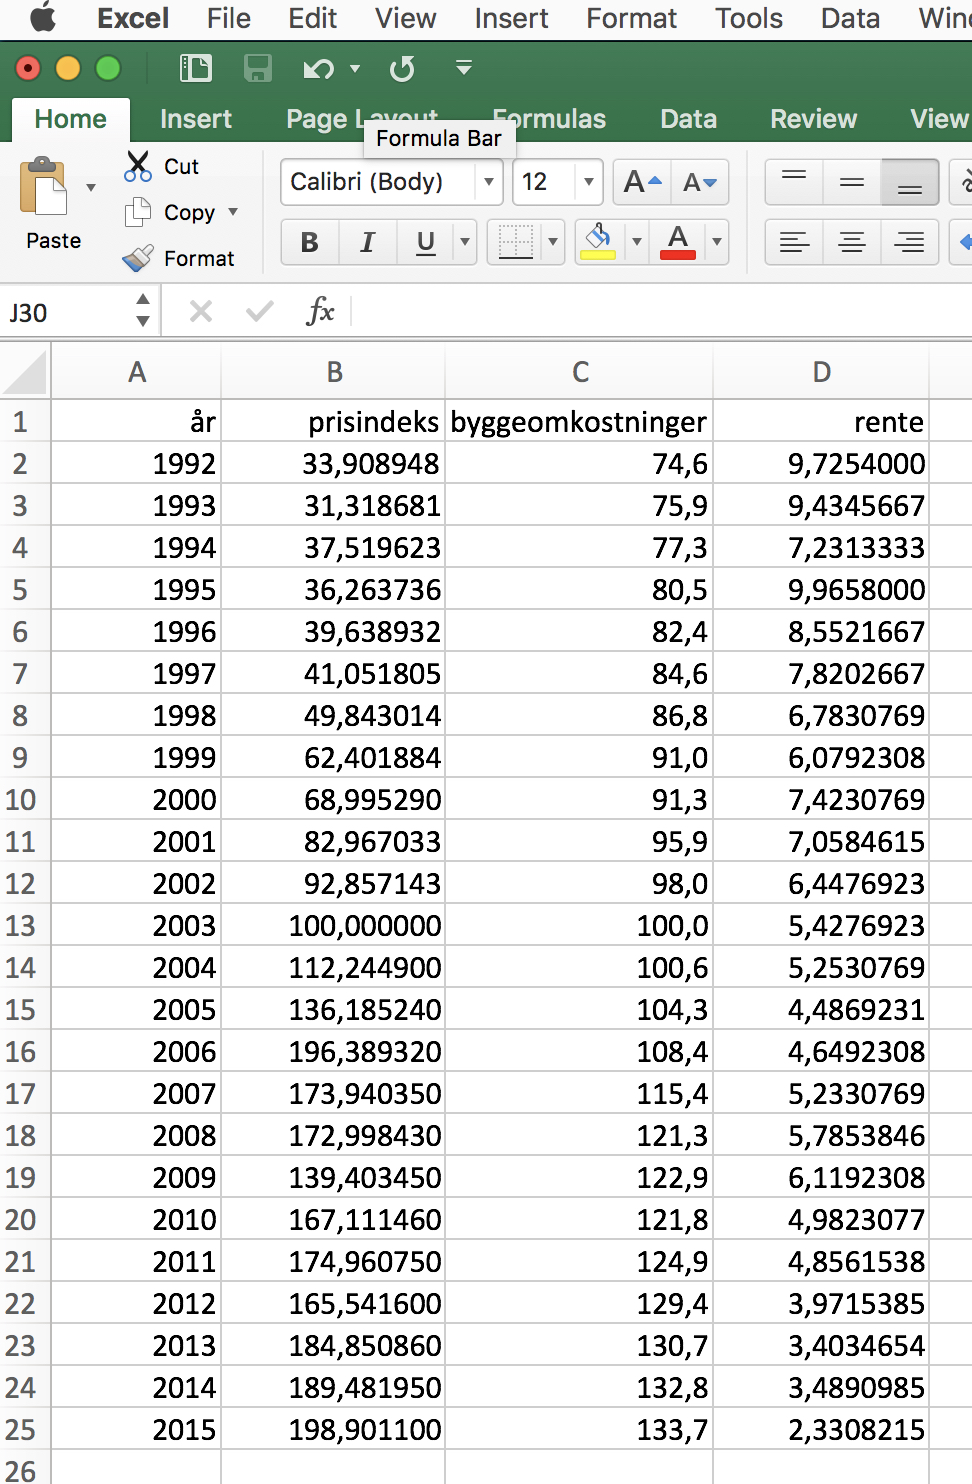
\includegraphics[height=12cm]{regression/images/data.JPG}
\end{center}
Hvis du selv ønsker at arbejde med dette datasæt, så kan det downloades via dette \href{https://gist.github.com/carsten-j/42595fb16fc646a22bf3f4bec1d81e59/archive/b45e8d1e5e14b83aa16daa652821a8d7b7a3b56d.zip}{link}.

I menuen under ``Tools'' finder man ``Data Analysis''. Hvis Data Analysis ikke er en del af menuen, så er her en \href{https://support.office.com/en-us/article/Load-the-Analysis-ToolPak-6a63e598-cd6d-42e3-9317-6b40ba1a66b4}{vejledning} til hvordan man får den installeret i Excel.
\begin{center}
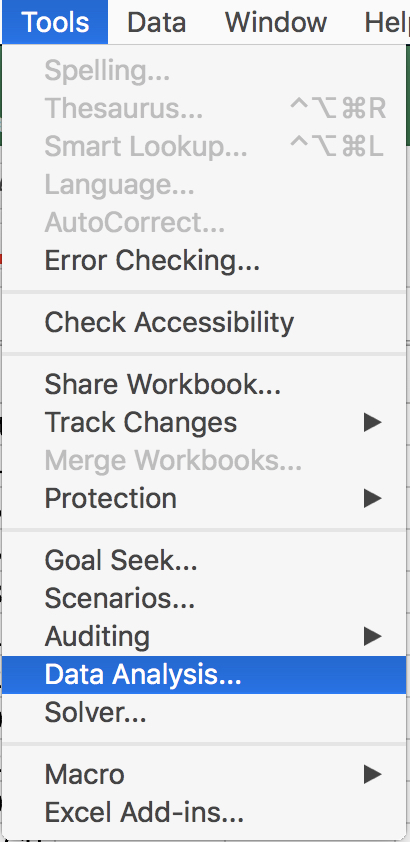
\includegraphics[height=8cm]{regression/images/menu.JPG}
\end{center}
og dernæst fås en oversigt over de forskellige analyseværktøjer. Vælg ``Regression''
\begin{center}
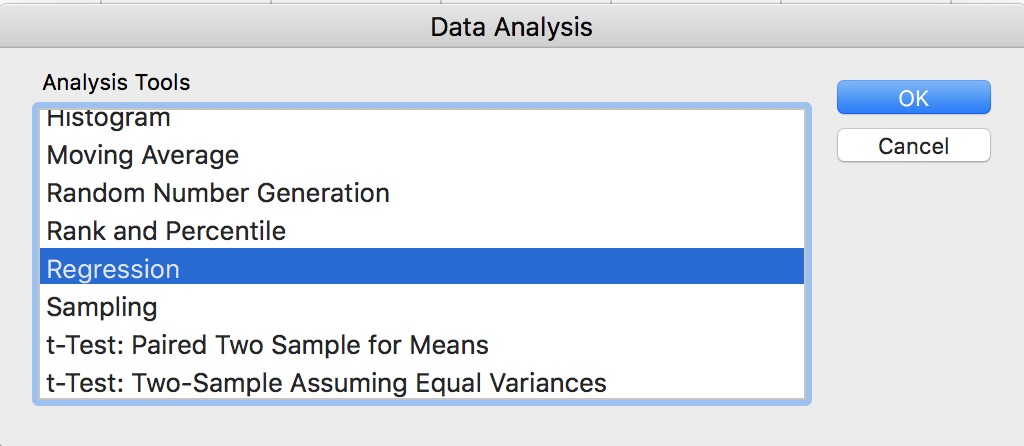
\includegraphics[height=5cm]{regression/images/analysisTools.JPG}
\end{center}
Så dukker denne regression menu op
\begin{center}\label{figure:regressionMenu}
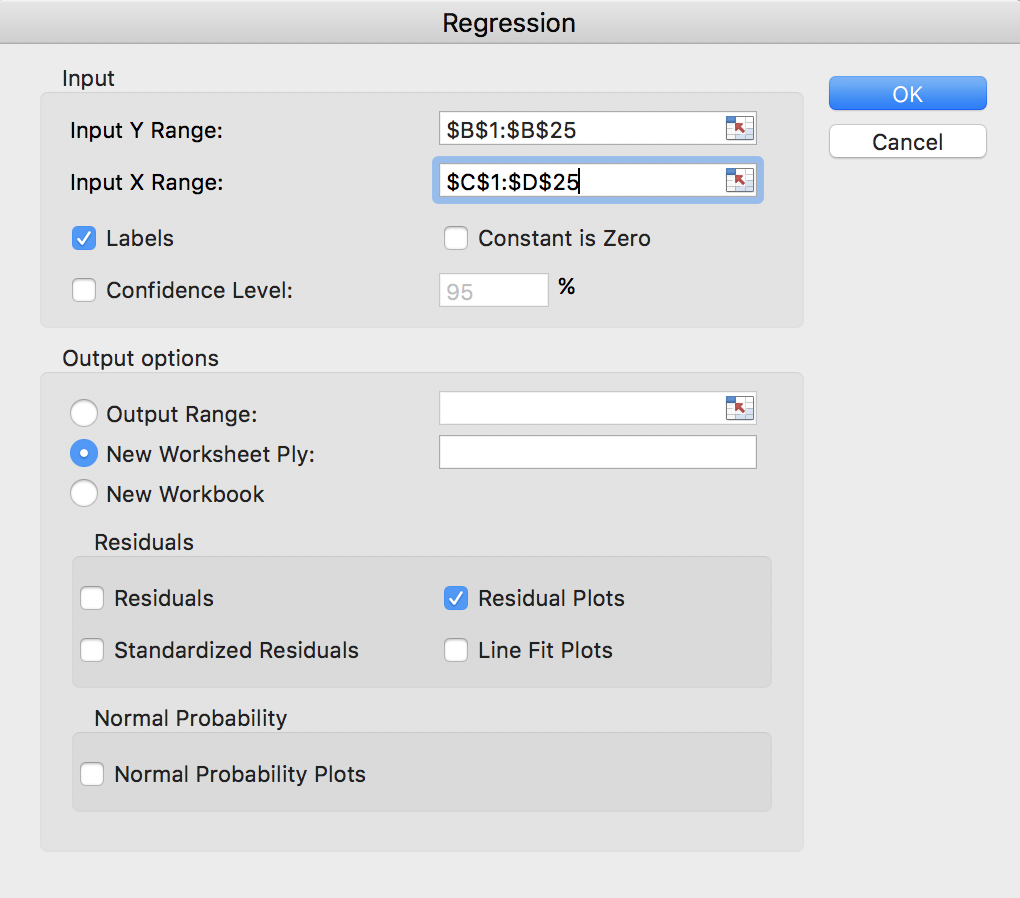
\includegraphics[height=10cm]{regression/images/regression.JPG}
\end{center}
Her har vi som ``Input Y Range'' valgt kolonnen med prisindeks (inkl.\ overskriften). Dette er vores afhængige variable. Dernæst har vi som ``Input X Range'' valgt kolonnerne med data for byggeomkostninger og renter (igen inkl.\ overskrift). Ved at sætte kryds i ``Labels'' checkboksen fortæller vi Excel, at vores valg af inputdata indeholder overskrifter. Det gør det nemmere at læse resultaterne. Som det sidste vælger vi også ``Residual Plots''.

Som udgangspunkt bliver alle resultater placeret i en nyt Excel sheet. Så er det lettere at slette dette sheet og begynde forfra, hvis man får behov for det.

Der er en masse output fra beregningen, men i første omgang fokuseres vi på regressionskoefficienterne
\begin{center}\label{figure:regressionCoefficients}
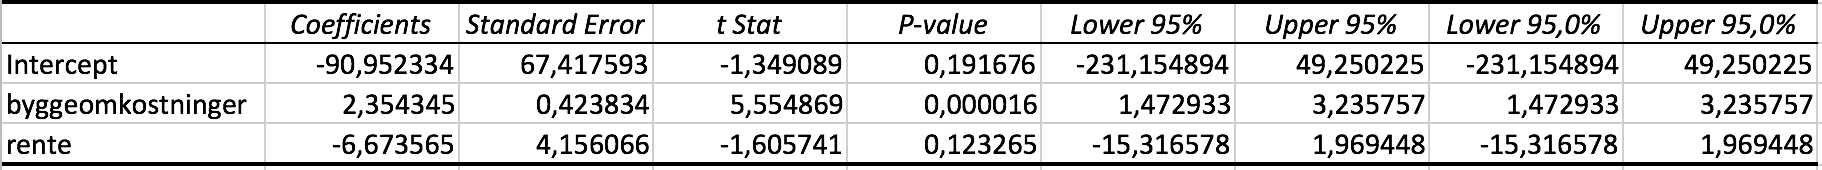
\includegraphics[width=16cm]{regression/images/regressionCoefficients.JPG}
\end{center}
Indsætter vi de fundne koefficienter i model \ref{eq:model} får vi regressionsligningen
\begin{displaymath}
  \textrm{prisindeks} = -90,95 + 2,35 * \textrm{byggeomkostninger} - 6,67 * \textrm{rente}
\end{displaymath}

Efter at have bestemt selve modellen kigger vi på tallene under overskriften ``Regression Statistics'':
\begin{center}\label{tabel:resultat}
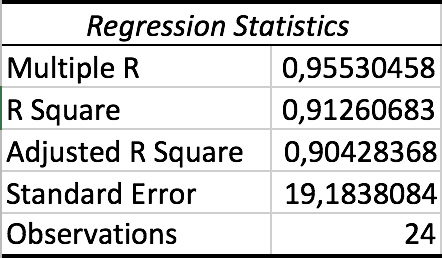
\includegraphics[height=2.5cm]{regression/images/resultat.JPG}
\end{center}
Her sætter vi fokus på Multiple R og R Square. På dansk kaldes disse to værdier for korrelations- og determinationskoefficienten.

\subsection{Korrelationskoefficienten}
Det er med Excel altid muligt at bestemme regressionskoefficienterne \(b_0,b_1,b_2,\ldots,b_p\), så spørgsmålet er mere, om det giver mening at forsøge at modellere en lineær sammenhæng mellem en afhængig variable og en eller flere forklarende variable. Det kan korrelationskoefficienten hjælpe os med at afklare. I Excel betegnes korrelationskoefficienten med ``Multiple R''. Men typisk bruger man blot betegnelsen R for korrelationskoefficienten.

\subsubsection{Fortolkning af korrelationskoefficienten}
Korrelation mellem to variable betyder, at hvis den ene variables ændre sig, så giver det en forudsigelig ændring i den anden variabel. Korrelationskoefficienten ligger altid mellem 0 og 1. Hvis den er 1, er der en deterministisk korrelation mellem variablene, dvs en ændring i den ene variabel vil helt sikkert medføre en ændring i den anden variable. Hvis værdien derimod er 0, så er der absolut ingen lineær sammenhæng mellem de to variable. Skematisk ser det ud som i tabel~\ref{tabel:correlation}.
\begin{table}[h]
\centering
\caption{Fortolkning af korrelationskoefficienten}
\label{tabel:correlation}
\begin{tabular}{|r|l|}
\hline
\multicolumn{1}{|l|}{R værdi} & Fortolkning                     \\ \hline
1,0                           & Perfekt lineær sammenhæng       \\ \hline
0,0                           & Absolut ingen lineær sammenhæng \\ \hline
0,9                           & Stærk lineær sammenhæng         \\ \hline
0,5                           & Moderat lineær sammenhæng       \\ \hline
0,2                           & Svag lineær sammenhæng          \\ \hline
\end{tabular}
\end{table}
\textbf{Bemærk} at en høj grad af korrelation på ingen måder kan bruges til at postulere en årsagssammenhæng (kausalitet) mellem variable. Se afsnittet TODO for mere information.

Hvis multipel lineær regression skal give mening, så \textit{skal} der være en lineær sammenhæng mellem den afhængige variable og de forklarende variable. Hvis vi kigger på eksemplet fra tidligere, jvf tabel~\ref{tabel:resultat}, så ser vi, at der her er en korrelationskoefficient på ca. 0,9553 og at der dermed i dette tilfælde er en korrelation mellem variable pris, byggeomkostninger og rente.

\subsubsection{Formel for korrelationskoefficienten for to uafhængige variable}
Den generelle formel for korrelationskoefficienten er kompliceret og involveret matrix beregninger. I tilfældet hvor vi kun har to uafhængige variable er det lidt nemmere at skrive formlen ned.
\begin{displaymath}\label{eq:correlation}
  R = \frac{\sqrt{r^2_{yx_1} + r^2_{yx_2} - 2r_{yx_1} r_{yx_2} r_{{x_1}x_2}}}{\sqrt{1 - r^2_{{x_1}x_2}}}
\end{displaymath}
hvor fx
\begin{displaymath}
  r_{{y}{x_1}} = \frac{\sum{(y - \overbar{y})(x_1 - \overbar{x_1})}}{(n-1)s_{{y}{x_1}}}
\end{displaymath}
og
\begin{displaymath}
  \overbar{y} = \frac{y_{i}}{n}, \quad \overbar{x_1} = \frac{x_{1i}}{n}, \quad s_{y} = \sqrt{\frac{\sum{(y_{i} - \overbar{y})^2}}{n-1}}, \quad s_{x_1} = \sqrt{\frac{\sum{(x_{1i} - \overbar{x_1})^2}}{n-1}}
\end{displaymath}
Størrelsen \(r_{{y}{x_1}}\) er dybest set korrelationskoefficienten mellem variablene \(y\) og \(x_1\). Når formlen \ref{eq:correlation} er mere kompleks skyldes det, at vi også er nød til at betragte korrelationen mellem \(y\) og \(x_2\) og mellem \(x_1\) og \(x_2\).

Pointen med at opskrive formlen er ikke, at du skal kunne regne korrelationskoefficienten i hånden. Pointen er derimod at kunne sammenligne med simpel regressionsanalyse. Hvis vi nu kun har en enkelt forklarende variable \(x_1\) og \(x_2=0\), så forsvinder de fleste led i formlen~\ref{tabel:correlation}. Tilbage bliver kun de led, hvor \(x_2\) ikke indgår, dvs
\begin{displaymath}
  R = \frac{\sqrt{r^2_{yx_1}}}{\sqrt{1}} = r_{yx_1}
\end{displaymath}
hvilket præcis er korrelationskoefficienten for simpel lineær regression mellem den afhængige variabel \(y\) og den forklarende variabel \(x_1\).

\subsection{Determinationskoefficienten}
I Excel hedder determinationskoefficienten ``R Square'', hvilket giver god mening, da formlen for determinationskoefficienten er kvadratet på korrelationskoefficienten, dvs
\begin{displaymath}
\mathrm{determinationskoefficienten} = R^2
\end{displaymath}
Man hører jænvligt alternative betegnelser for determinationskoefficienten som fx for\-kla\-rings\-grad\-en eller tilpasningsgraden.

\subsubsection{Alternativ formel}
Der findes en alternativ formel for \(R^2\) - som naturligvis giver samme værdi. Det er lettest at beregne determinationskoefficienten som kvadratet på korrelationskoefficienten men den alternative formel gør det nemmere at fortolke determinationskoefficienten.

Vi har tidligere set, at SSE er forskellen mellem de fittede og observerede værdier. På samme måde kan man definere SSR som værende forskellen på de fittede værdier og gennemsnittet af observationerne, dvs
\begin{displaymath}
    \textrm{SSR} = \sum_{i=1}^{n} \Big( \widehat{y_i} - \bar{y} \Big)
\end{displaymath}
Definitionen på den totale ``Sum of Squares'' er
\begin{displaymath}
    \textrm{SST} = \textrm{SSR} + \textrm{SSE}
\end{displaymath}

For observationerne \(y_i\) definerer man den totale ``sum of squares'' som
\begin{displaymath}
    \textrm{SS}_T = \sum_{i=1}^{n} \Big( y_i - \bar{y} \Big )
\end{displaymath}
hvor \(\bar{y}\) er gennemsnittet af \(y_i\)'erne. Tilsvarende defineres  ``sum of squares'' for regressions. Den alternative formel for \(R^2\) er
\begin{displaymath}
    R^2 = \frac{SSR}{SST}
\end{displaymath}

\subsubsection{Fortolkning af Determinationskoefficienten}
Vi har altså ligningen
\begin{align}
    \textrm{SST}              &= \textrm{SSR} + \textrm{SSE} \\
    \textrm{Totale variation} &= \textrm{Forklaret variation} \\
                              &+ \textrm{Uforklaret variation}
\end{align}

så formlen for \(R^2\) er forholdet mellem den forklarede og totale variation i modellen. Så jo tættere \(R^2\) er på 1, desto mere variation er forklaret af modellen. Hvis \(R^2\) kommer meget tæt på 1 eller ligefrem bliver 1, så er der dog grund til ekstra omtanke. Se mere i afsnit ..

\subsection{Residual plot}
Det sidste output fra Excel som vi kigger nærmere på er residual plots. Husk at vi i menu \ref{figure:regressionMenu} sætte kryds ved ``Residual Plots''. Dette giver os disse to residual plots
\begin{center}
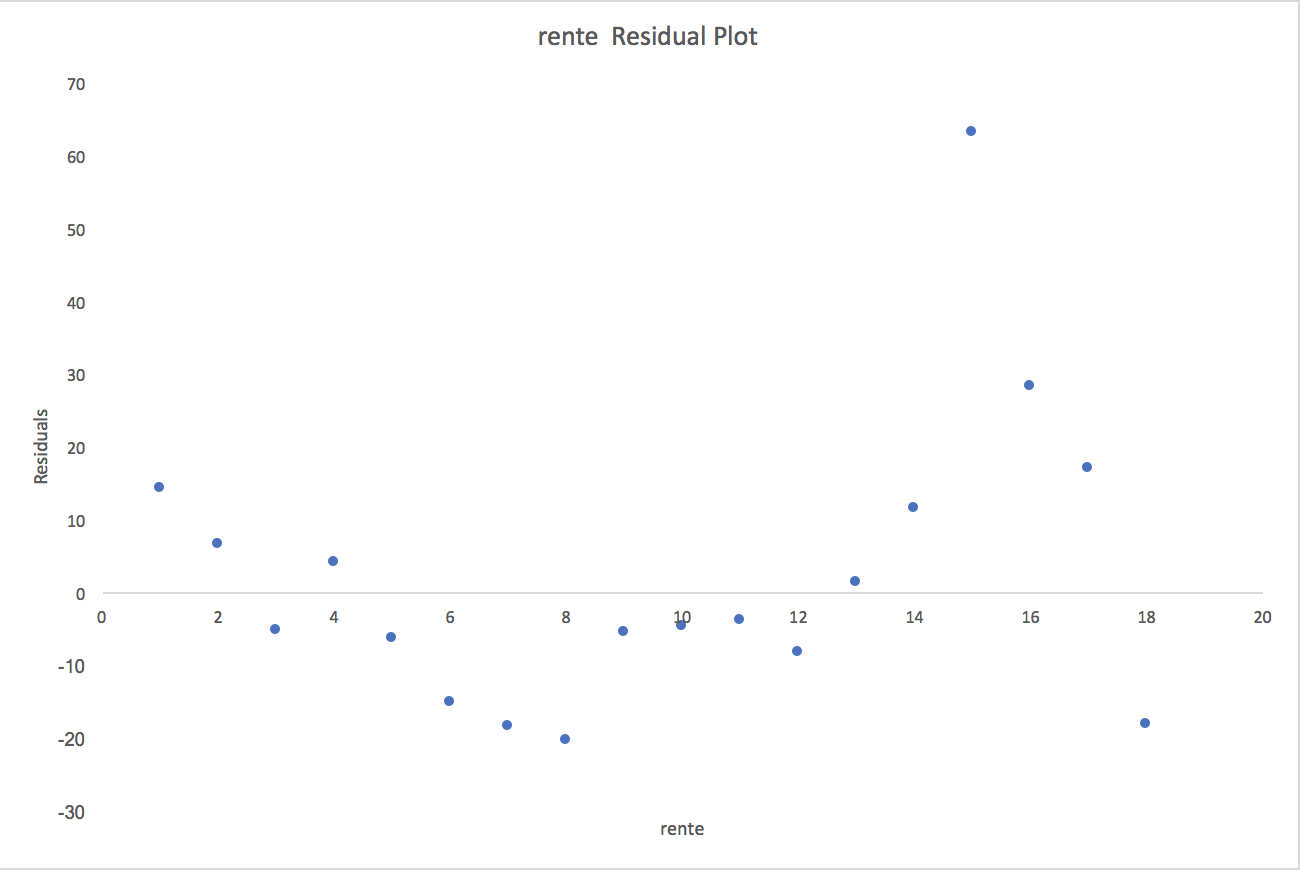
\includegraphics[width=12cm]{regression/images/residualplot1.JPG}
\end{center}
\begin{center}
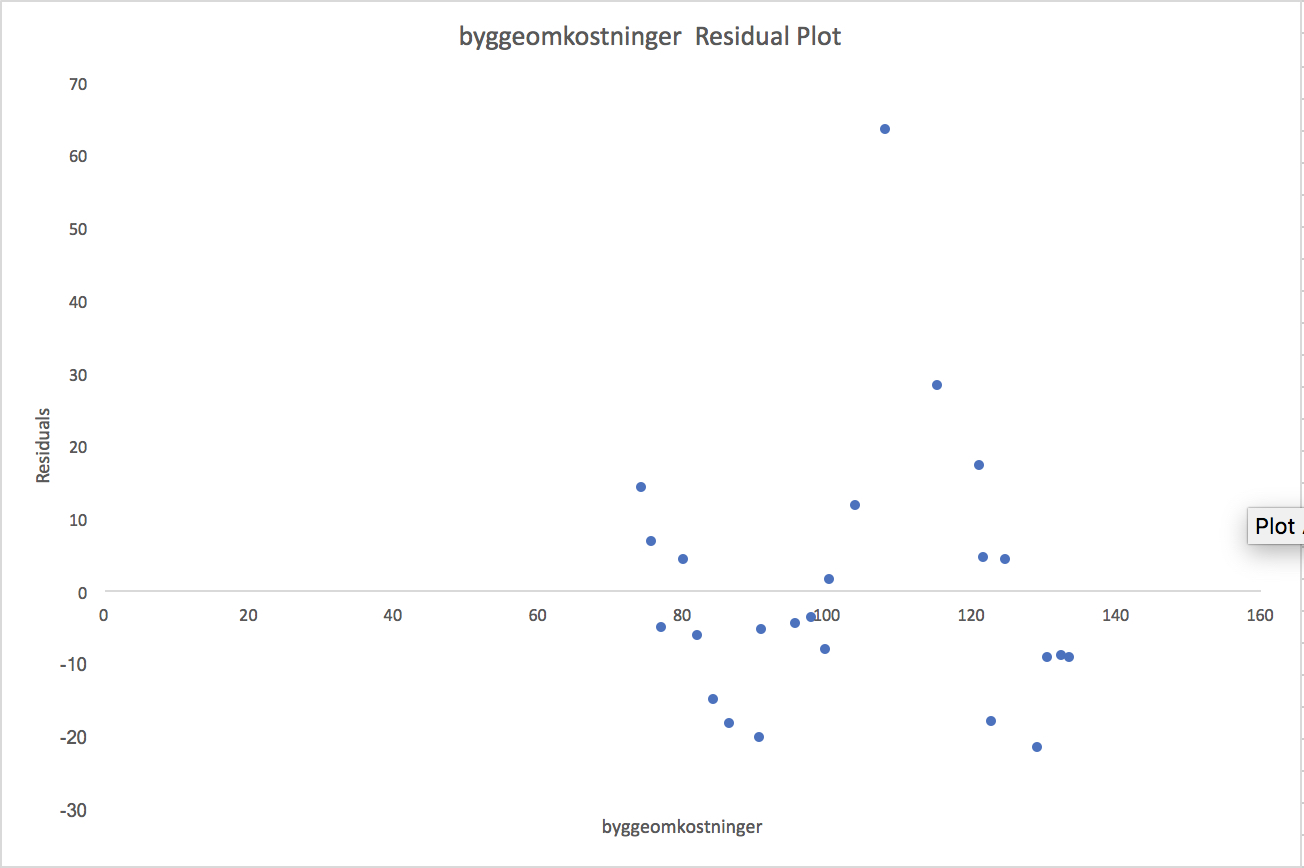
\includegraphics[width=12cm]{regression/images/residualplot2.JPG}
\end{center}
Husk at residualerne er forskellen mellem de fittede og observerede værdier. Hvis residual plottene virker helt tilfældige, så giver den mening at bruge en lineær model. Kan man derimod spotte en trend i residual plottet, som fx en ret linie eller et polynomium, så giver det ikke mening med en lineær model. Begge ovenstående plots virker tilfældige, så i vores eksempel giver det mening at bruge en lineær model.

\subsection{Konfidensinterval for parametre}
Vi har tidligere behandlet konfidensintervaller for middelværdier og sandsynslighedparameteren. Man kan også bestemme konfidensintervaller for regressionskoefficienterne. Faktisk er de en del af output, når man bruger Excel til regressionsanalyse. Kig igen på tabel \ref{figure:regressionCoefficients} som indeholdt regressionskoefficienterne. Der er nogle kolonner med overskriften ``Lower 95\%'' og ``Upper 95\%''. Tallene i disse kolonner er nedre og øvre grænse for et \(100\% - 95\% = 5\%\) konfidensinterval omkring regressionskoefficienterne.

Det kan være lidt forvirrende, at kolonnerne ``Lower 95\%'' og ``Upper 95\%'' er gentaget to gange med samme værdier. Hvis du kigger på menuen i figur ... kan du se, at man kan sætte kryds i ``Confidence Level'' og indtaste et konfidensniveau. Hvis man gør dette med fx 1\% så får man kolonnerne v ``Lower 95\%'' og ``Upper 95\%'' samt  ``Lower 99\%'' og ``Upper 99\%''. Dvs som udgangspunkt får man altid 5\% konfidensinterval med som resultat og derudover kan man få et ekstra interval efter eget valg.

\subsubsection{Formel for konfidensinterval}
Formel for \(1 - \alpha\) konfidensintervallet for de enkelte regressionskoefficienter er
\begin{displaymath}
    b_i \pm t(v, 1 - \alpha / 2) \textrm{se}(b_i)
\end{displaymath}
Her er
\begin{itemize}
    \item \(t\) t-test funktionen
    \item \(v\) er antallet af observationer minus antallet af regressionskoefficienter og
    \item se\((b_i)\) er ``standard error'' for \(b_i\)
\end{itemize}
Størrelsen se\((b_i)\) er svær at regne ud i hånden og formlen involvere matrix beregninger. Men kig igen på tabel \ref{figure:regressionCoefficients}. Faktisk er standard fejlen er del af output fra Excel. t-test funktionen er indbygget i Excel under navnet T.INV.2T.

Som eksempel kan vi regne et 90\% konfidensinterval for \(b_1\). Her er \(v=24-3=21\), \(\alpha=0,1\), se\((b_i) = 0,42\) og \(b_1=2,35\), så konfidensintervallet bliver
\begin{align}
    \Big[2,35 - \textrm{T.INV.2T(0,1;21)} * 0,42 ;  2,35 + \textrm{T.INV.2T(0,1;21)} * 0,42 \Big] &= \\
    \Big[2,35 - 1,72 * 0,42 ;  2,35 + 1,72 * 0,42 \Big] &= \\
    \Big[2,35 - 1,72 * 0,42 ;  2,35 + 1,72 * 0,42 \Big] &= \\
    \Big[1,6276 ; 3,0724\Big]
\end{align}

\subsection{Avancerede emner}
Disse emner falder udenfor pensum men for den nysgerrige er her en kort introduktion til emner, som er vigtige i forbindelse med regressionsanalyse.

\subsubsection{Udforskende dataanalyse}
Indenfor området data science arbejder man en del med udforskende dataanalyse. Dette indebærer, at man før man kaster sig hovedkuls ud i at vælge den ene eller anden model, så tager man sig tid til at undersøge data nærmere. Det giver fx ikke mening at bruge en lineær regressionsmodel, hvis man på en graf kan se, at der umuligt kan være en lineær sammenhæng mellem en afhængig variable og en forklarende variabel. Det er ikke helt nemt at afgøre om der kan være en lineær sammenhæng mellem en afhængig variable og \textit{flere} forklarende variable. Så på nuværende tidspunkt er det bedste man kan gøre at undersøge om det er plausibelt at der er en lineær sammenhæng mellem ens afhængige varibel og de forklarende variable en for en.

Der findes et klassisk eksempel under navnet Anscombes kvartet, hvor  statistikeren Francis Anscombe viser fire forskellige datasæt med næsten identiske deskriptive statistikker (som fx middelværdi og varians), men når man laver en graf for hver af datasættene, så for man meget forskellige grafer.
\begin{center}
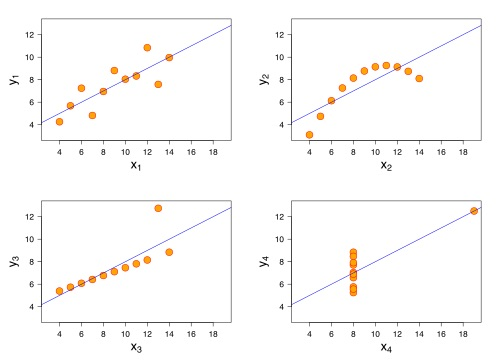
\includegraphics[width=12cm]{regression/images/Anscombes.JPG}
\end{center}
Grafen er fra ``Anscombe's quartet 3.svg. (2016, December 14). Wikimedia Commons, the free media repository'', hvor den original fil findes her \url{https://commons.wikimedia.org/w/index.php?title=File:Anscombe%27s_quartet_3.svg&oldid=226250329}.

\subsubsection{Model udvælgelse og multicollinearitet}
Lad os sige, at vi har en model med en afhængig variabel og fire forklarende variable.
\begin{displaymath}
    y = b_0 + b_1 x_2 + b_2 x_2 + b_3 x_3 + b_4 x_4
\end{displaymath}
Hvordan kan vi være sikre på, at dette er den rigtige model. Måske skulle vi hellere udelade \(x_2\) eller \(x_3\) eller både \(x_2\) og \(x_3\). Sådanne spørgsmål forsøger man at besvare indenfor emnet model udvælgelse. Der findes en række statistiske tests som kan være med til at afgøre, om det er en god ide eller ej, at inkludere de enkelte variable.

Når man vælger de forklarende variable skal man også passe på med multicollinearitet. Dvs at ingen af de forklarende variable må kunne skrives som lineære funktioner af de øvrige forklarende variable. I eksempel med fire forklarende variable kan vi fx ikke have at
\begin{displaymath}
    x_2 = x_1 + x_4
\end{displaymath}

\subsubsection{Justeret \(R^2\)}
I forlængelse af forrige afsnit om model udvælgelse er det værd at bemærke følgende. Hvis vi tilføjer flere forklarende variable til vores model, så vil det stort set næsten altid være sådan, at værdien af \(R^2\) bliver større. Betyder det, at det altid er godt at tilføje flere forklarende variable til ens model? Hvis vi har \(n\) observationer, så kan vi jo vælge en model med \(n-1\) forklarende variable. Dette vil ofte give en værdi af \(R^2\) meget tæt på 1. Så må det jo være en god model! Svaret er nej. Derfor bruger man ofte ikke determinationskoefficienten \(R^2\) men en værdi som kaldes justeret \(R^2\), når man skal se på om det giver mening at tilføje en ekstra variable til modellen.

\subsubsection{Korrelation og kausalitet}
Når vi arbejder med lineær regressionsanalyse leder vi efter korrelationer mellem den afhængige variable og en række forklarende variable. Det er meget vigtigt at have for øje, at en lineær sammenhæng mellem en række variable ikke er ensbetydende med en kausalitet eller årsagssammenhæng mellem de samme variable. På \href{http://videnskab.dk/kultur-samfund/korrelation-eller-kausalitet-hvornaar-er-der-en-aarsagssammenhaeng}{Videnskab.dk} kan du finde en let tilgængelig artikel om korrelation og kausalitet og lære mere om forskellen samt hvad man skal passe på med.
